\subfloat[$Calcul~graphique~de~l'autocorrélation~de~p(\frac{t}{T_s})$]
{
	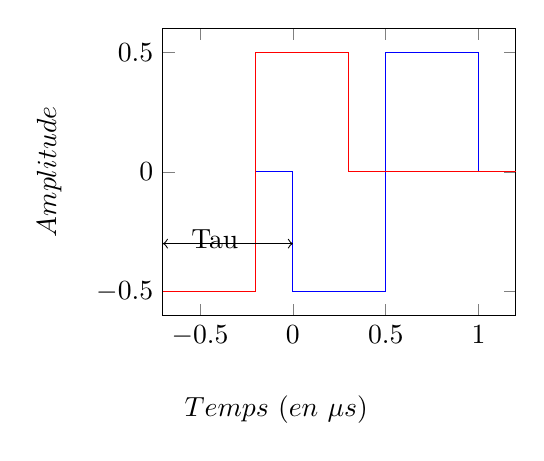
\begin{tikzpicture}
		\begin{axis}[
				xmin=-0.7,xmax=1.2,
				ymin=-0.6,ymax=0.6,
				xlabel={$Temps~(en~\mu s)$},
				ylabel={$Amplitude$},
				xlabel style={anchor=north, yshift=-0.4cm, xshift=-0.8cm},
				ylabel style={yshift=0.2cm},
				width=0.50\textwidth
			]
			\addplot[color=blue,mark=none] coordinates {
				(-0.2,0)
				(0, 0)
				(0, -0.5)
				(0.5, -0.5)
				(0.5, 0.5)
				(1, 0.5)
				(1, 0)
				(1.2, 0)
			};
			\addplot[color=red,mark=none] coordinates {
				(-0.7, -0.5)
				(-0.2, -0.5)
				(-0.2, 0.5)
				(0.3, 0.5)
				(0.3, 0)
				(1.2, 0)
			};
			\addplot[color=black,<->] coordinates {
				(-0.7, -0.3)
				(0, -0.3)
			};
			\node at (axis cs:-0.6,-0.2) [anchor=north west] {Tau};
		\end{axis}
	\end{tikzpicture}
}\hfill{}\subfloat[$\tilde{R_{s_{l}}}(\frac{\tau}{T_s})$]
{
	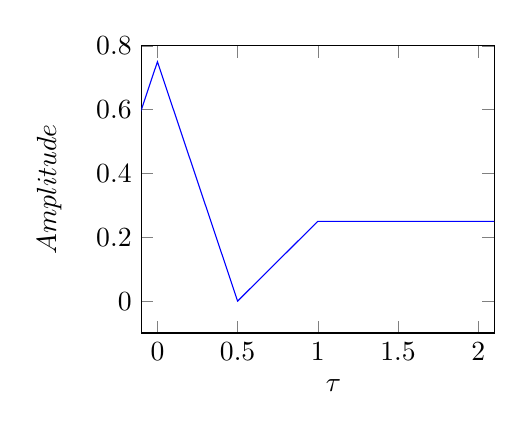
\begin{tikzpicture}
		\begin{axis}[
				xmin=-0.1,xmax=2.1,
				ymin=-0.1,ymax=0.8,
				xlabel={$\tau$},
				ylabel={$Amplitude$},
				xlabel style={xshift=0.2cm},
				ylabel style={yshift=0.2cm},
				width=0.50\textwidth
			]
			\addplot[color=blue,mark=none] coordinates {
				(-0.5, 0)
				(0, 0.75)
				(0.5, 0)
				(1, 0.25)
				(2.1, 0.25)
			};
		\end{axis}
	\end{tikzpicture}
}
